% Options for packages loaded elsewhere
\PassOptionsToPackage{unicode}{hyperref}
\PassOptionsToPackage{hyphens}{url}
%
\documentclass[
  12pt,
]{article}
\title{Comparison of Physical Characteristics, Avian Clutch Size, and
Mating Tactics}
\usepackage{etoolbox}
\makeatletter
\providecommand{\subtitle}[1]{% add subtitle to \maketitle
  \apptocmd{\@title}{\par {\large #1 \par}}{}{}
}
\makeatother
\subtitle{\url{https://github.com/jcf55/Fahrenholz_Costes_ENV872_EDA_FinalProject}}
\author{Lydie Costes and Jackie Fahrenholz}
\date{}

\usepackage{amsmath,amssymb}
\usepackage{lmodern}
\usepackage{iftex}
\ifPDFTeX
  \usepackage[T1]{fontenc}
  \usepackage[utf8]{inputenc}
  \usepackage{textcomp} % provide euro and other symbols
\else % if luatex or xetex
  \usepackage{unicode-math}
  \defaultfontfeatures{Scale=MatchLowercase}
  \defaultfontfeatures[\rmfamily]{Ligatures=TeX,Scale=1}
  \setmainfont[]{Times New Roman}
\fi
% Use upquote if available, for straight quotes in verbatim environments
\IfFileExists{upquote.sty}{\usepackage{upquote}}{}
\IfFileExists{microtype.sty}{% use microtype if available
  \usepackage[]{microtype}
  \UseMicrotypeSet[protrusion]{basicmath} % disable protrusion for tt fonts
}{}
\makeatletter
\@ifundefined{KOMAClassName}{% if non-KOMA class
  \IfFileExists{parskip.sty}{%
    \usepackage{parskip}
  }{% else
    \setlength{\parindent}{0pt}
    \setlength{\parskip}{6pt plus 2pt minus 1pt}}
}{% if KOMA class
  \KOMAoptions{parskip=half}}
\makeatother
\usepackage{xcolor}
\IfFileExists{xurl.sty}{\usepackage{xurl}}{} % add URL line breaks if available
\IfFileExists{bookmark.sty}{\usepackage{bookmark}}{\usepackage{hyperref}}
\hypersetup{
  pdftitle={Comparison of Physical Characteristics, Avian Clutch Size, and Mating Tactics},
  pdfauthor={Lydie Costes and Jackie Fahrenholz},
  hidelinks,
  pdfcreator={LaTeX via pandoc}}
\urlstyle{same} % disable monospaced font for URLs
\usepackage[margin=2.54cm]{geometry}
\usepackage{color}
\usepackage{fancyvrb}
\newcommand{\VerbBar}{|}
\newcommand{\VERB}{\Verb[commandchars=\\\{\}]}
\DefineVerbatimEnvironment{Highlighting}{Verbatim}{commandchars=\\\{\}}
% Add ',fontsize=\small' for more characters per line
\usepackage{framed}
\definecolor{shadecolor}{RGB}{248,248,248}
\newenvironment{Shaded}{\begin{snugshade}}{\end{snugshade}}
\newcommand{\AlertTok}[1]{\textcolor[rgb]{0.94,0.16,0.16}{#1}}
\newcommand{\AnnotationTok}[1]{\textcolor[rgb]{0.56,0.35,0.01}{\textbf{\textit{#1}}}}
\newcommand{\AttributeTok}[1]{\textcolor[rgb]{0.77,0.63,0.00}{#1}}
\newcommand{\BaseNTok}[1]{\textcolor[rgb]{0.00,0.00,0.81}{#1}}
\newcommand{\BuiltInTok}[1]{#1}
\newcommand{\CharTok}[1]{\textcolor[rgb]{0.31,0.60,0.02}{#1}}
\newcommand{\CommentTok}[1]{\textcolor[rgb]{0.56,0.35,0.01}{\textit{#1}}}
\newcommand{\CommentVarTok}[1]{\textcolor[rgb]{0.56,0.35,0.01}{\textbf{\textit{#1}}}}
\newcommand{\ConstantTok}[1]{\textcolor[rgb]{0.00,0.00,0.00}{#1}}
\newcommand{\ControlFlowTok}[1]{\textcolor[rgb]{0.13,0.29,0.53}{\textbf{#1}}}
\newcommand{\DataTypeTok}[1]{\textcolor[rgb]{0.13,0.29,0.53}{#1}}
\newcommand{\DecValTok}[1]{\textcolor[rgb]{0.00,0.00,0.81}{#1}}
\newcommand{\DocumentationTok}[1]{\textcolor[rgb]{0.56,0.35,0.01}{\textbf{\textit{#1}}}}
\newcommand{\ErrorTok}[1]{\textcolor[rgb]{0.64,0.00,0.00}{\textbf{#1}}}
\newcommand{\ExtensionTok}[1]{#1}
\newcommand{\FloatTok}[1]{\textcolor[rgb]{0.00,0.00,0.81}{#1}}
\newcommand{\FunctionTok}[1]{\textcolor[rgb]{0.00,0.00,0.00}{#1}}
\newcommand{\ImportTok}[1]{#1}
\newcommand{\InformationTok}[1]{\textcolor[rgb]{0.56,0.35,0.01}{\textbf{\textit{#1}}}}
\newcommand{\KeywordTok}[1]{\textcolor[rgb]{0.13,0.29,0.53}{\textbf{#1}}}
\newcommand{\NormalTok}[1]{#1}
\newcommand{\OperatorTok}[1]{\textcolor[rgb]{0.81,0.36,0.00}{\textbf{#1}}}
\newcommand{\OtherTok}[1]{\textcolor[rgb]{0.56,0.35,0.01}{#1}}
\newcommand{\PreprocessorTok}[1]{\textcolor[rgb]{0.56,0.35,0.01}{\textit{#1}}}
\newcommand{\RegionMarkerTok}[1]{#1}
\newcommand{\SpecialCharTok}[1]{\textcolor[rgb]{0.00,0.00,0.00}{#1}}
\newcommand{\SpecialStringTok}[1]{\textcolor[rgb]{0.31,0.60,0.02}{#1}}
\newcommand{\StringTok}[1]{\textcolor[rgb]{0.31,0.60,0.02}{#1}}
\newcommand{\VariableTok}[1]{\textcolor[rgb]{0.00,0.00,0.00}{#1}}
\newcommand{\VerbatimStringTok}[1]{\textcolor[rgb]{0.31,0.60,0.02}{#1}}
\newcommand{\WarningTok}[1]{\textcolor[rgb]{0.56,0.35,0.01}{\textbf{\textit{#1}}}}
\usepackage{graphicx}
\makeatletter
\def\maxwidth{\ifdim\Gin@nat@width>\linewidth\linewidth\else\Gin@nat@width\fi}
\def\maxheight{\ifdim\Gin@nat@height>\textheight\textheight\else\Gin@nat@height\fi}
\makeatother
% Scale images if necessary, so that they will not overflow the page
% margins by default, and it is still possible to overwrite the defaults
% using explicit options in \includegraphics[width, height, ...]{}
\setkeys{Gin}{width=\maxwidth,height=\maxheight,keepaspectratio}
% Set default figure placement to htbp
\makeatletter
\def\fps@figure{htbp}
\makeatother
\setlength{\emergencystretch}{3em} % prevent overfull lines
\providecommand{\tightlist}{%
  \setlength{\itemsep}{0pt}\setlength{\parskip}{0pt}}
\setcounter{secnumdepth}{5}
\usepackage{booktabs}
\usepackage{longtable}
\usepackage{array}
\usepackage{multirow}
\usepackage{wrapfig}
\usepackage{float}
\usepackage{colortbl}
\usepackage{pdflscape}
\usepackage{tabu}
\usepackage{threeparttable}
\usepackage{threeparttablex}
\usepackage[normalem]{ulem}
\usepackage{makecell}
\usepackage{xcolor}
\ifLuaTeX
  \usepackage{selnolig}  % disable illegal ligatures
\fi

\begin{document}
\maketitle

\newpage
\tableofcontents 
\newpage
\listoftables 
\listoffigures 
\newpage

\hypertarget{rationale-and-research-questions}{%
\section{Rationale and Research
Questions}\label{rationale-and-research-questions}}

According to the study from which this data was extracted, avian body
size and the evolution of birds over time is a highly debated subject
matter. Generally, there is agreement around the idea that body size of
bird species relates to other characteristics. This project intends to
explore the correlation between body size and other characteristics in
our data.

First, we ask the question if female tail size predicts clutch size.
Tail length has a significant impact on control and agility (Evans
1999). Longer tails increase crash risk as well as reduces the ability
to maneuver (Evans 1999). We believe that this may have an overall
negative impact on clutch size, as birds with longer tail lengths may be
less efficient at collecting food for their young.

Second, we will explore interactions between male tail length and
methods of display, mating system, and resource sharing systems. Tail
length likely has a negative impact on navigation, and collecting food,
while having a positive impact on sexual display. Physical
characteristics of males are evaluated by females in search of a mate,
but the importance of tail length may vary greatly by species.

\hypertarget{dataset-information}{%
\section{Dataset Information}\label{dataset-information}}

Our dataset consists of data that was collected starting in 2005 and was
last updated in January of 2007. Data for this collection come from
regions that include:

\begin{itemize}
\tightlist
\item
  Western Palearctic
\item
  Neararctic
\item
  Africa
\item
  Australia
\item
  New Zealand
\item
  Antarctica
\end{itemize}

The complete dataset (represented below by the variable \texttt{birds})
includes 41 variables and represents 125 families. According to the
metadata, the majority of this information was gathered from
ornithological handbooks, with some data obtained from personal
communications with authors who published information on species bird
groups. More information on the sources used can be found at:
\url{https://esapubs.org/archive/ecol/E088/096/metadata.htm} (also in
/Data/Raw in the .tex file)

\newpage

\hypertarget{exploration-of-raw-data}{%
\section{Exploration of Raw Data}\label{exploration-of-raw-data}}

\begin{Shaded}
\begin{Highlighting}[]
\CommentTok{\#dimensions}
\FunctionTok{dim}\NormalTok{(birds)}
\end{Highlighting}
\end{Shaded}

\begin{verbatim}
## [1] 3769   41
\end{verbatim}

\begin{Shaded}
\begin{Highlighting}[]
\CommentTok{\#column names}
\FunctionTok{colnames}\NormalTok{(birds)}
\end{Highlighting}
\end{Shaded}

\begin{verbatim}
##  [1] "Family"           "Species_number"   "Species_name"     "English_name"    
##  [5] "Subspecies"       "M_mass"           "M_mass_N"         "F_mass"          
##  [9] "F_mass_N"         "unsexed_mass"     "unsexed_mass_N"   "M_wing"          
## [13] "M_wing_N"         "F_wing"           "F_wing_N"         "Unsexed_wing"    
## [17] "Unsexed_wing_N"   "M_tarsus"         "M_tarsus_N"       "F_tarsus"        
## [21] "F_tarsus_N"       "Unsexed_tarsus"   "Unsexed_tarsus_N" "M_bill"          
## [25] "M_bill_N"         "F_bill"           "F_bill_N"         "Unsexed_bill"    
## [29] "Unsexed_bill_N"   "M_tail"           "M_tail_N"         "F_tail"          
## [33] "F_tail_N"         "Unsexed_tail"     "Unsexed_tail_N"   "Clutch_size"     
## [37] "Egg_mass"         "Mating_System"    "Display"          "Resource"        
## [41] "References"
\end{verbatim}

\begin{Shaded}
\begin{Highlighting}[]
\CommentTok{\#variable types}
\FunctionTok{str}\NormalTok{(birds)}
\end{Highlighting}
\end{Shaded}

\begin{verbatim}
## 'data.frame':    3769 obs. of  41 variables:
##  $ Family          : int  115 101 116 116 116 116 116 116 116 116 ...
##  $ Species_number  : int  5351 3964 5402 5398 5400 5401 5396 5405 5404 5397 ...
##  $ Species_name    : chr  "Acanthagenys rufogularis" "Acanthisitta chloris" "Acanthiza chrysorrhoa" "Acanthiza ewingii" ...
##  $ English_name    : chr  "Spiny-cheeked Honeyeater" "Rifleman" "Yellow-rumped Thornbill" "Tasmanian Thornbill" ...
##  $ Subspecies      : chr  "-999" "-999" "leighi" "ewingii" ...
##  $ M_mass          : num  47.1 5.6 9.4 7.2 7.2 5.8 6.8 7.6 6.5 7.4 ...
##  $ M_mass_N        : int  4 33 25 16 43 16 10 25 27 37 ...
##  $ F_mass          : num  41.4 7 9.8 6.7 6.9 5.7 6.7 7.4 6.3 6.5 ...
##  $ F_mass_N        : int  5 20 16 19 76 12 7 27 23 20 ...
##  $ unsexed_mass    : num  -999 -999 -999 -999 -999 -999 -999 -999 -999 -999 ...
##  $ unsexed_mass_N  : int  -999 -999 -999 -999 -999 -999 -999 -999 -999 -999 ...
##  $ M_wing          : num  113.1 47.8 57.8 52.7 48.9 ...
##  $ M_wing_N        : int  25 10 25 21 28 29 11 36 25 52 ...
##  $ F_wing          : num  107.5 51.4 57.6 51 47 ...
##  $ F_wing_N        : num  21 10 26 22 26 25 7 26 29 30 ...
##  $ Unsexed_wing    : num  -999 -999 -999 -999 -999 -999 -999 -999 -999 -999 ...
##  $ Unsexed_wing_N  : int  -999 -999 -999 -999 -999 -999 -999 -999 -999 -999 ...
##  $ M_tarsus        : num  26.2 19.1 17.7 21.3 18 18.4 18.5 17.5 17.4 20.3 ...
##  $ M_tarsus_N      : int  10 10 23 21 28 29 11 36 25 51 ...
##  $ F_tarsus        : num  25.7 19.7 17.4 21.7 17.8 17.6 18.4 17.5 17.3 19.3 ...
##  $ F_tarsus_N      : int  5 7 24 23 25 25 7 25 27 29 ...
##  $ Unsexed_tarsus  : num  -999 -999 -999 -999 -999 -999 -999 -999 -999 -999 ...
##  $ Unsexed_tarsus_N: int  -999 -999 -999 -999 -999 -999 -999 -999 -999 -999 ...
##  $ M_bill          : num  26.8 13.2 11.9 11 11.3 9.7 11.6 10.2 10 11 ...
##  $ M_bill_N        : int  8 6 24 21 27 28 11 26 24 51 ...
##  $ F_bill          : num  25.5 14.4 11.7 10.9 11.4 9.6 11.2 9.9 10 10.5 ...
##  $ F_bill_N        : num  10 7 26 23 25 24 7 26 28 29 ...
##  $ Unsexed_bill    : num  -999 -999 -999 -999 -999 -999 -999 -999 -999 -999 ...
##  $ Unsexed_bill_N  : int  -999 -999 -999 -999 -999 -999 -999 -999 -999 -999 ...
##  $ M_tail          : num  113.4 23.3 40.8 47.8 36.3 ...
##  $ M_tail_N        : int  25 10 28 21 34 28 11 36 14 51 ...
##  $ F_tail          : num  106.4 22.1 39.3 46.8 35.4 ...
##  $ F_tail_N        : int  21 7 26 23 55 25 6 26 10 30 ...
##  $ Unsexed_tail    : num  -999 -999 -999 -999 -999 -999 -999 -999 -999 -999 ...
##  $ Unsexed_tail_N  : int  -999 -999 -999 -999 -999 -999 -999 -999 -999 -999 ...
##  $ Clutch_size     : num  2.2 4 3.5 3.5 3 3 2.5 3 3 3 ...
##  $ Egg_mass        : num  5.45 1.34 1.44 1.46 1.35 0.93 -999 1.32 1.34 1.4 ...
##  $ Mating_System   : int  2 2 2 2 2 -999 -999 2 2 2 ...
##  $ Display         : int  3 1 1 1 -999 1 -999 2 -999 1 ...
##  $ Resource        : int  2 2 1 0 1 1 -999 0 -999 2 ...
##  $ References      : chr  "1, 21" "21" "1, 22, 31 " "22, 31" ...
\end{verbatim}

\newpage

\hypertarget{data-wrangling}{%
\section{Data Wrangling}\label{data-wrangling}}

\begin{Shaded}
\begin{Highlighting}[]
\CommentTok{\# make sure family column is named correctly}
\FunctionTok{colnames}\NormalTok{(birds)[}\DecValTok{1}\NormalTok{] }\OtherTok{\textless{}{-}} \StringTok{"Family"}

\CommentTok{\# Convert {-}999 to NAs and add genus column}
\NormalTok{birds }\OtherTok{\textless{}{-}}\NormalTok{ birds }\SpecialCharTok{\%\textgreater{}\%}
  \FunctionTok{na\_if}\NormalTok{(., }\SpecialCharTok{{-}}\DecValTok{999}\NormalTok{) }\SpecialCharTok{\%\textgreater{}\%}
  \FunctionTok{separate}\NormalTok{(Species\_name, }
           \AttributeTok{sep =} \StringTok{" "}\NormalTok{, }
           \AttributeTok{into =} \FunctionTok{c}\NormalTok{(}\StringTok{"Genus"}\NormalTok{, }\StringTok{"Sp"}\NormalTok{), }
           \AttributeTok{remove =} \ConstantTok{FALSE}\NormalTok{)}

\CommentTok{\# Subset to columns we are interested in}
\NormalTok{birds.subset }\OtherTok{\textless{}{-}}\NormalTok{ birds }\SpecialCharTok{\%\textgreater{}\%}
  \FunctionTok{select}\NormalTok{(Family, Species\_name, Genus, F\_mass, M\_mass, }
\NormalTok{         F\_tail, M\_tail, Clutch\_size, Mating\_System, }
\NormalTok{         Display, Resource)}

\CommentTok{\# Group male tail length by mating system to graph later}
\NormalTok{birds.mating.tail }\OtherTok{\textless{}{-}}\NormalTok{ birds.subset }\SpecialCharTok{\%\textgreater{}\%}
  \FunctionTok{group\_by}\NormalTok{(Mating\_System) }\SpecialCharTok{\%\textgreater{}\%}
  \FunctionTok{summarise}\NormalTok{(}\AttributeTok{M\_tail =} \FunctionTok{mean}\NormalTok{(M\_tail, }\AttributeTok{na.rm =} \ConstantTok{TRUE}\NormalTok{))}

\CommentTok{\# This function allows calculation of mode for categorical variables}
\NormalTok{Mode }\OtherTok{\textless{}{-}} \ControlFlowTok{function}\NormalTok{(x) \{}
\NormalTok{  ux }\OtherTok{\textless{}{-}} \FunctionTok{unique}\NormalTok{(x) }
\NormalTok{  ux[}\FunctionTok{which.max}\NormalTok{(}\FunctionTok{tabulate}\NormalTok{(}\FunctionTok{match}\NormalTok{(x, ux)))]}
\NormalTok{\}}

\CommentTok{\# Group by family, average by mean or mode}
\NormalTok{birds.family }\OtherTok{\textless{}{-}}\NormalTok{ birds.subset }\SpecialCharTok{\%\textgreater{}\%}
  \FunctionTok{group\_by}\NormalTok{(Family) }\SpecialCharTok{\%\textgreater{}\%} 
  \FunctionTok{summarise}\NormalTok{(}\AttributeTok{F\_mass =} \FunctionTok{mean}\NormalTok{(F\_mass, }\AttributeTok{na.rm =} \ConstantTok{TRUE}\NormalTok{),}
            \AttributeTok{M\_mass =} \FunctionTok{mean}\NormalTok{(M\_mass, }\AttributeTok{na.rm =} \ConstantTok{TRUE}\NormalTok{),}
            \AttributeTok{F\_tail =} \FunctionTok{mean}\NormalTok{(F\_tail, }\AttributeTok{na.rm =} \ConstantTok{TRUE}\NormalTok{),}
            \AttributeTok{M\_tail =} \FunctionTok{mean}\NormalTok{(M\_tail, }\AttributeTok{na.rm =} \ConstantTok{TRUE}\NormalTok{),}
            \AttributeTok{Clutch\_size =} \FunctionTok{mean}\NormalTok{(Clutch\_size, }\AttributeTok{na.rm =} \ConstantTok{TRUE}\NormalTok{),}
            \AttributeTok{Common\_Mating\_System =} \FunctionTok{Mode}\NormalTok{(Mating\_System),}
            \AttributeTok{Common\_Display =} \FunctionTok{Mode}\NormalTok{(Display),}
            \AttributeTok{Common\_Resource =} \FunctionTok{Mode}\NormalTok{(Resource)) }\SpecialCharTok{\%\textgreater{}\%}
  \FunctionTok{filter}\NormalTok{(}\SpecialCharTok{!}\FunctionTok{is.na}\NormalTok{(Clutch\_size), }\SpecialCharTok{!}\FunctionTok{is.na}\NormalTok{(F\_tail), }
         \SpecialCharTok{!}\FunctionTok{is.na}\NormalTok{(F\_mass), }\SpecialCharTok{!}\FunctionTok{is.na}\NormalTok{(M\_tail))}

\CommentTok{\# Set categorical variables as factors}
\NormalTok{birds.subset}\SpecialCharTok{$}\NormalTok{Family }\OtherTok{\textless{}{-}} \FunctionTok{as.factor}\NormalTok{(birds.subset}\SpecialCharTok{$}\NormalTok{Family)}
\NormalTok{birds.subset}\SpecialCharTok{$}\NormalTok{Mating\_System }\OtherTok{\textless{}{-}} \FunctionTok{as.factor}\NormalTok{(birds.subset}\SpecialCharTok{$}\NormalTok{Mating\_System)}
\NormalTok{birds.subset}\SpecialCharTok{$}\NormalTok{Display }\OtherTok{\textless{}{-}} \FunctionTok{as.factor}\NormalTok{(birds.subset}\SpecialCharTok{$}\NormalTok{Display)}
\NormalTok{birds.subset}\SpecialCharTok{$}\NormalTok{Resource }\OtherTok{\textless{}{-}} \FunctionTok{as.factor}\NormalTok{(birds.subset}\SpecialCharTok{$}\NormalTok{Resource)}

\CommentTok{\# Write the csv file into our Processed data folder}
\FunctionTok{write.csv}\NormalTok{(birds.subset, }\AttributeTok{file =} \StringTok{"../Data/Processed/birds\_subset.csv"}\NormalTok{)}
\FunctionTok{write.csv}\NormalTok{(birds.family, }\AttributeTok{file =} \StringTok{"../Data/Processed/birds\_family.csv"}\NormalTok{)}
\end{Highlighting}
\end{Shaded}

\newpage

\hypertarget{exploration-of-processed-data}{%
\section{Exploration of Processed
Data}\label{exploration-of-processed-data}}

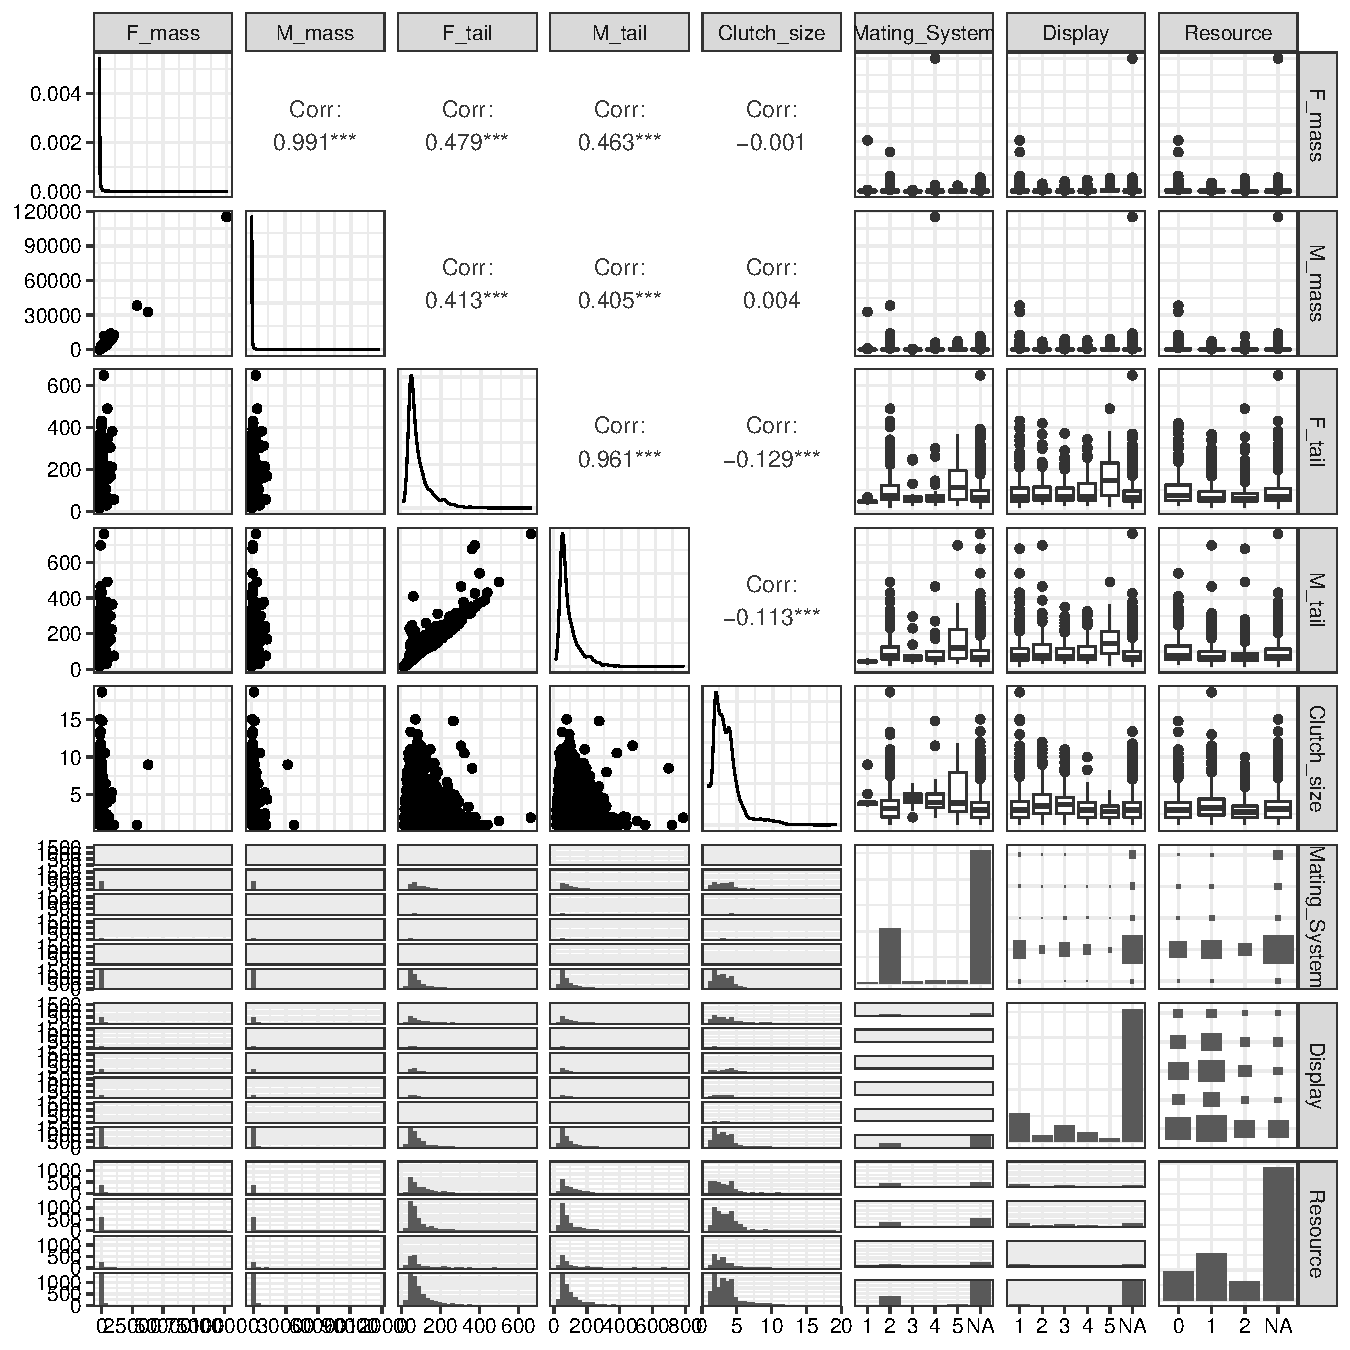
\includegraphics{Project_Code_files/figure-latex/gg exploration-1.pdf}

\newpage
\begin{table}

\caption{\label{tab:summary table}Summary Statistics for Continuous Variables}
\centering
\begin{tabular}[t]{l|r|r|r|r|r|r|r|r}
\hline
  & vars & n & mean & sd & min & max & range & se\\
\hline
F\_mass & 1 & 2706 & 411.472616 & 2320.49997 & 1.8 & 100000.0 & 99998.2 & 44.6085053\\
\hline
M\_mass & 2 & 2822 & 436.692275 & 2585.46747 & 2.0 & 115000.0 & 114998.0 & 48.6699134\\
\hline
F\_tail & 3 & 2352 & 88.340901 & 59.91081 & 15.4 & 647.5 & 632.1 & 1.2353402\\
\hline
M\_tail & 4 & 2390 & 92.410126 & 64.27592 & 15.8 & 762.0 & 746.2 & 1.3147688\\
\hline
Clutch\_size & 5 & 2392 & 3.448037 & 1.88880 & 1.0 & 18.6 & 17.6 & 0.0386194\\
\hline
\end{tabular}
\end{table}

\newpage

As part of our exploration, we ran a regression to assess how correlated
male and female tail lengths are.

\begin{verbatim}
## 
## Call:
## lm(formula = M_tail ~ F_tail, data = birds.subset)
## 
## Residuals:
##    Min     1Q Median     3Q    Max 
## -46.84  -3.21  -1.27   0.85 345.40 
## 
## Coefficients:
##             Estimate Std. Error t value Pr(>|t|)    
## (Intercept) 1.226565   0.652716   1.879   0.0603 .  
## F_tail      1.033250   0.006115 168.974   <2e-16 ***
## ---
## Signif. codes:  0 '***' 0.001 '**' 0.01 '*' 0.05 '.' 0.1 ' ' 1
## 
## Residual standard error: 17.76 on 2348 degrees of freedom
##   (1419 observations deleted due to missingness)
## Multiple R-squared:  0.924,  Adjusted R-squared:  0.924 
## F-statistic: 2.855e+04 on 1 and 2348 DF,  p-value: < 2.2e-16
\end{verbatim}

The answer is very much so (p \textless{} 0.001, Adjusted R\^{}2 =
0.924).

\newpage

Below, although male and female tail lengths are highly correlated, some
male tail lengths are unusually higher in comparison with female tail
lengths. These species may be ones where males have adapted longer tails
via sexual selection.

\begin{figure}
\centering
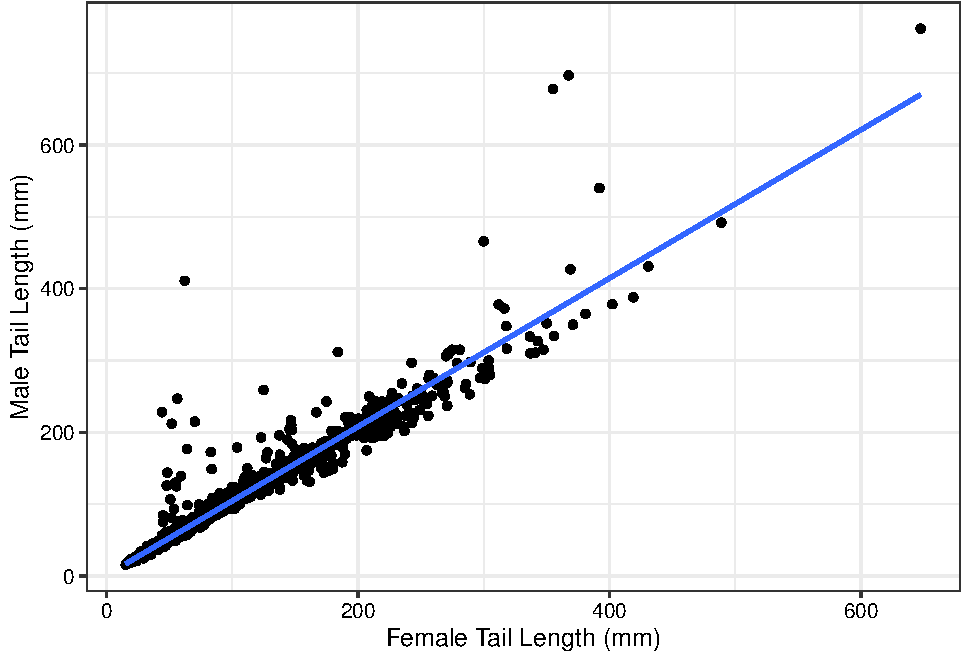
\includegraphics{Project_Code_files/figure-latex/r exploratory_plots_3-1.pdf}
\caption{The Relationship between Female and Male Tail Length}
\end{figure}

\newpage

To visualize the relationship between male and female tail length
another way, here are the distributions of tail length sorted by family
and divided by sex.

\begin{figure}
\centering
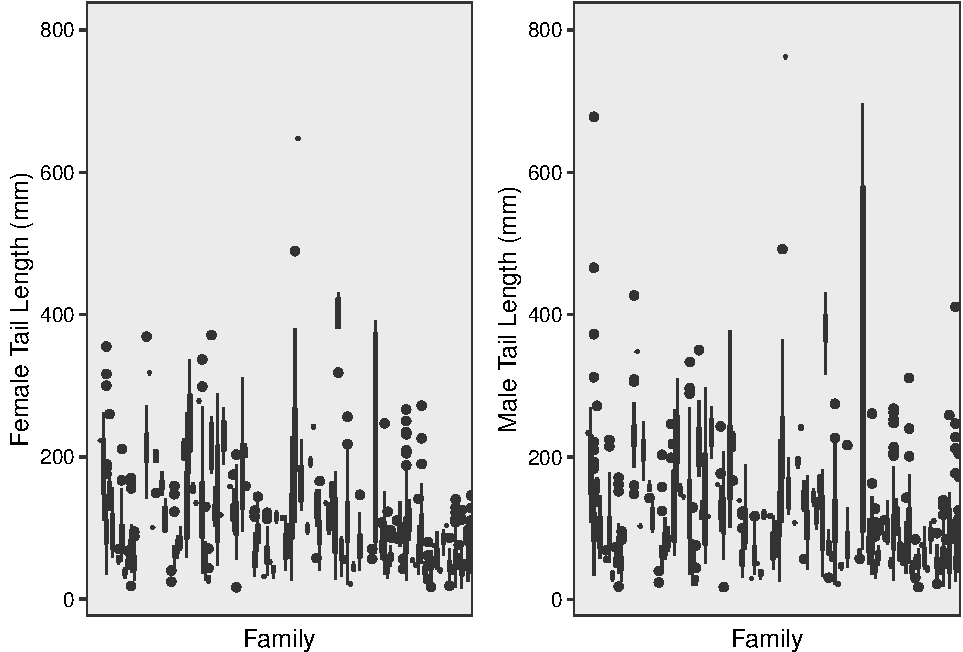
\includegraphics{Project_Code_files/figure-latex/r exploratory_plots_1-1.pdf}
\caption{Exploratory Plots of Tail Length by Sex and Family}
\end{figure}

\newpage

\hypertarget{analysis}{%
\section{Analysis}\label{analysis}}

To test our hypotheses using our subset data \texttt{birds.subset}, we
will conduct a linear regression and an analysis of variance (ANOVA).
Our first research question will be answered using a linear regression,
while our second will be addressed with an ANOVA. Results will be
clearly stated in words, and supplemented using graphing visualizations.

\hypertarget{question-1-does-female-tail-length-predict-clutch-size}{%
\subsection{Question 1: Does female tail length predict clutch
size?}\label{question-1-does-female-tail-length-predict-clutch-size}}

\(H_0\) : There is no significant difference between female tail length
and clutch size.

\(H_A\) : There is a significant difference between female tail length
and clutch size.

Prior to conducting this analysis, it was identified that there is a
strong correlation between female mass and female tail length. This
makes sense: in general, bigger birds will have longer tails. We
therefore included the mass variable in our model, in order to measure
the effect of tail on clutch size while controlling for the effect of
mass.

\begin{verbatim}
## 
## Call:
## lm(formula = Clutch_size ~ F_tail * F_mass)
## 
## Residuals:
##     Min      1Q  Median      3Q     Max 
## -4.9660 -1.2529 -0.2852  0.7347 11.9351 
## 
## Coefficients:
##                    Estimate    Std. Error t value  Pr(>|t|)    
## (Intercept)    3.8970630035  0.0920673618  42.328   < 2e-16 ***
## F_tail        -0.0038295564  0.0009331300  -4.104 0.0000426 ***
## F_mass         0.0002587737  0.0000979394   2.642   0.00832 ** 
## F_tail:F_mass -0.0000010753  0.0000004436  -2.424   0.01546 *  
## ---
## Signif. codes:  0 '***' 0.001 '**' 0.01 '*' 0.05 '.' 0.1 ' ' 1
## 
## Residual standard error: 1.891 on 1642 degrees of freedom
##   (2123 observations deleted due to missingness)
## Multiple R-squared:  0.02398,    Adjusted R-squared:  0.02219 
## F-statistic: 13.45 on 3 and 1642 DF,  p-value: 0.00000001141
\end{verbatim}

\begin{verbatim}
##        F_tail        F_mass F_tail:F_mass 
##      1.564475      4.086442      4.876822
\end{verbatim}

\begin{figure}
\centering
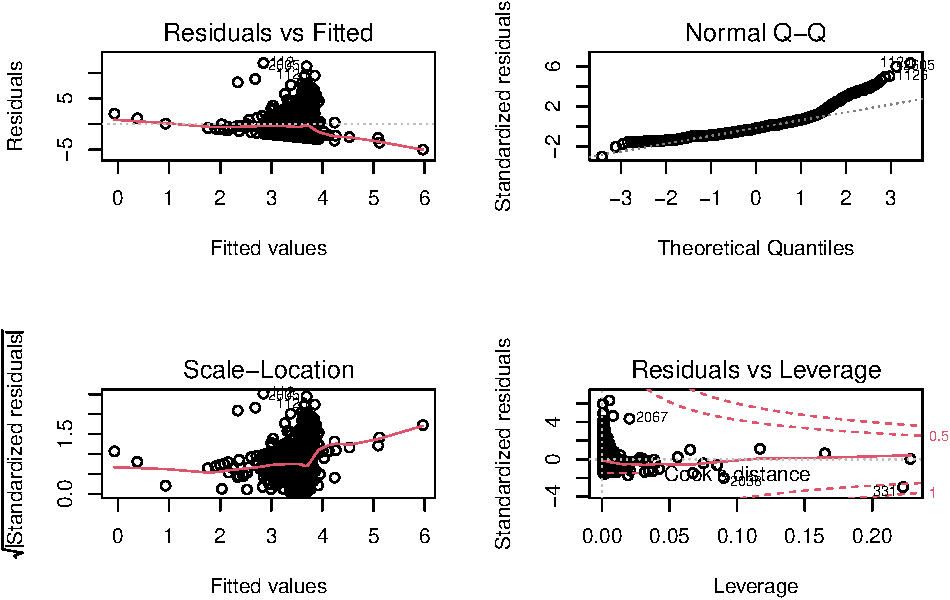
\includegraphics{Project_Code_files/figure-latex/q-1_residuals-1.pdf}
\caption{Residual Plots for Question 1}
\end{figure}

\newpage

Below, clutch size declines with increasing female tail length.

\begin{figure}
\centering
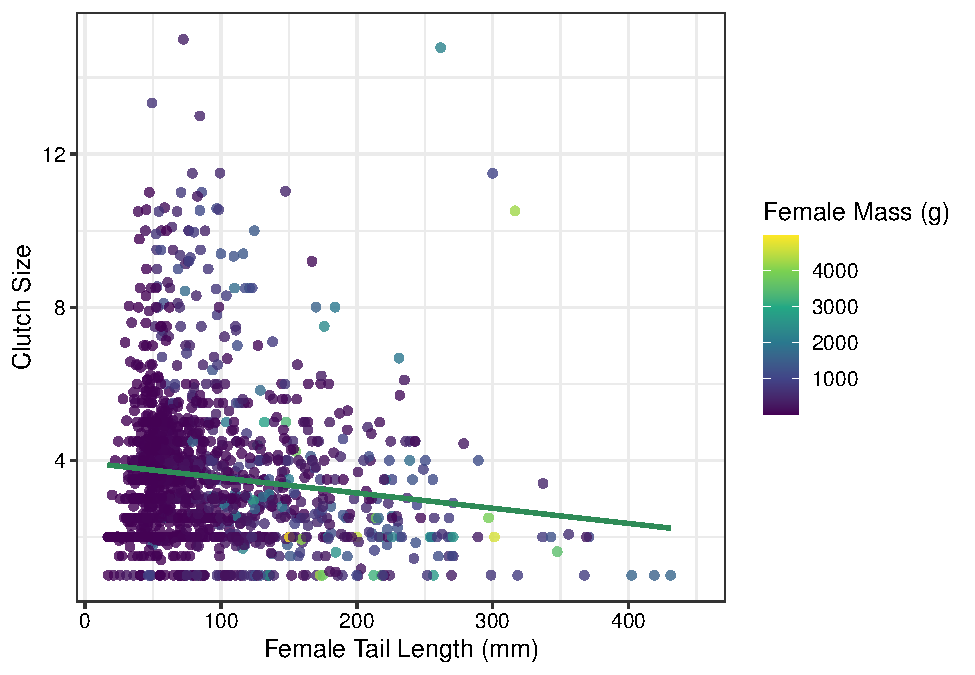
\includegraphics{Project_Code_files/figure-latex/q-1_plot_main-1.pdf}
\caption{Female Tail Length vs Clutch Size}
\end{figure}

\newpage

\hypertarget{question-2-does-male-tail-length-relate-to-mating-approaches}{%
\subsection{Question 2: Does male tail length relate to mating
approaches?}\label{question-2-does-male-tail-length-relate-to-mating-approaches}}

\(H_0\) : Mating system and display behavior do not predict tail size.

\(H_A\) : Mating system and/or display behavior do predict tail size.

First, test for normality and equal variance:

\begin{verbatim}
## 
##  Shapiro-Wilk normality test
## 
## data:  birds.subset$M_tail
## W = 0.75655, p-value < 2.2e-16
\end{verbatim}

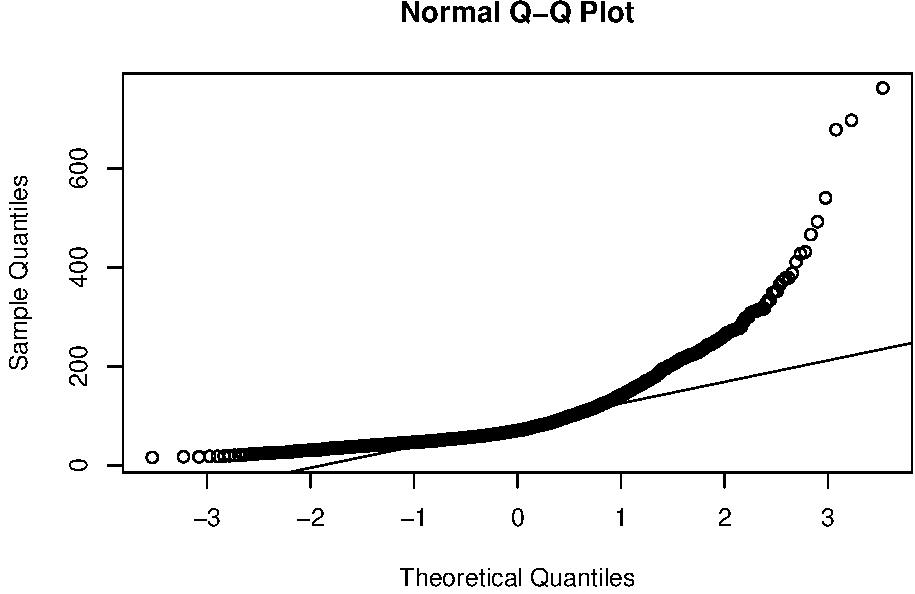
\includegraphics{Project_Code_files/figure-latex/question_2_part_1-1.pdf}

\begin{verbatim}
## 
##  Bartlett test of homogeneity of variances
## 
## data:  M_tail by Display
## Bartlett's K-squared = 71.043, df = 4, p-value = 0.00000000000001367
\end{verbatim}

\begin{verbatim}
## 
##  Bartlett test of homogeneity of variances
## 
## data:  M_tail by Mating_System
## Bartlett's K-squared = 102.13, df = 4, p-value < 2.2e-16
\end{verbatim}

\newpage

Next, run model:

\begin{Shaded}
\begin{Highlighting}[]
\NormalTok{mating.anova }\OtherTok{\textless{}{-}} \FunctionTok{aov}\NormalTok{(}\AttributeTok{data =}\NormalTok{ birds.subset, M\_tail }\SpecialCharTok{\textasciitilde{}}\NormalTok{ Mating\_System }\SpecialCharTok{*}\NormalTok{ Display }\SpecialCharTok{*}\NormalTok{ Resource)}
\FunctionTok{summary}\NormalTok{(mating.anova)}
\end{Highlighting}
\end{Shaded}

\begin{verbatim}
##                                 Df  Sum Sq Mean Sq F value            Pr(>F)
## Mating_System                    4   59317   14829   3.548           0.00737
## Display                          4  164931   41233   9.865 0.000000129331941
## Resource                         2   18622    9311   2.228           0.10914
## Mating_System:Display           11  377637   34331   8.214 0.000000000000544
## Mating_System:Resource           3   13812    4604   1.102           0.34832
## Display:Resource                 8   35663    4458   1.067           0.38570
## Mating_System:Display:Resource   4   12473    3118   0.746           0.56109
## Residuals                      393 1642577    4180                          
##                                   
## Mating_System                  ** 
## Display                        ***
## Resource                          
## Mating_System:Display          ***
## Mating_System:Resource            
## Display:Resource                  
## Mating_System:Display:Resource    
## Residuals                         
## ---
## Signif. codes:  0 '***' 0.001 '**' 0.01 '*' 0.05 '.' 0.1 ' ' 1
## 3339 observations deleted due to missingness
\end{verbatim}

\newpage

Because not everything was significant, we used a nested model approach
to reduce the model until all components were significant.

\begin{Shaded}
\begin{Highlighting}[]
\NormalTok{mating.anova.final }\OtherTok{\textless{}{-}} \FunctionTok{aov}\NormalTok{(}\AttributeTok{data =}\NormalTok{ birds.subset, M\_tail }\SpecialCharTok{\textasciitilde{}}\NormalTok{ Mating\_System }\SpecialCharTok{*}\NormalTok{ Display)}
\FunctionTok{summary}\NormalTok{(mating.anova.final)}
\end{Highlighting}
\end{Shaded}

\begin{verbatim}
##                        Df  Sum Sq Mean Sq F value     Pr(>F)    
## Mating_System           4  135625   33906   7.198 0.00001259 ***
## Display                 4  148286   37071   7.870 0.00000386 ***
## Mating_System:Display  12  229022   19085   4.052 0.00000526 ***
## Residuals             455 2143223    4710                       
## ---
## Signif. codes:  0 '***' 0.001 '**' 0.01 '*' 0.05 '.' 0.1 ' ' 1
## 3293 observations deleted due to missingness
\end{verbatim}

\begin{Shaded}
\begin{Highlighting}[]
\CommentTok{\#Grouping with Tukey HSD}
\NormalTok{anova.group }\OtherTok{\textless{}{-}} \FunctionTok{HSD.test}\NormalTok{(mating.anova}\FloatTok{.4}\NormalTok{, }\StringTok{"M\_tail"}\NormalTok{, }\AttributeTok{group =} \ConstantTok{TRUE}\NormalTok{)}
\NormalTok{anova.group}
\end{Highlighting}
\end{Shaded}

\begin{figure}
\centering
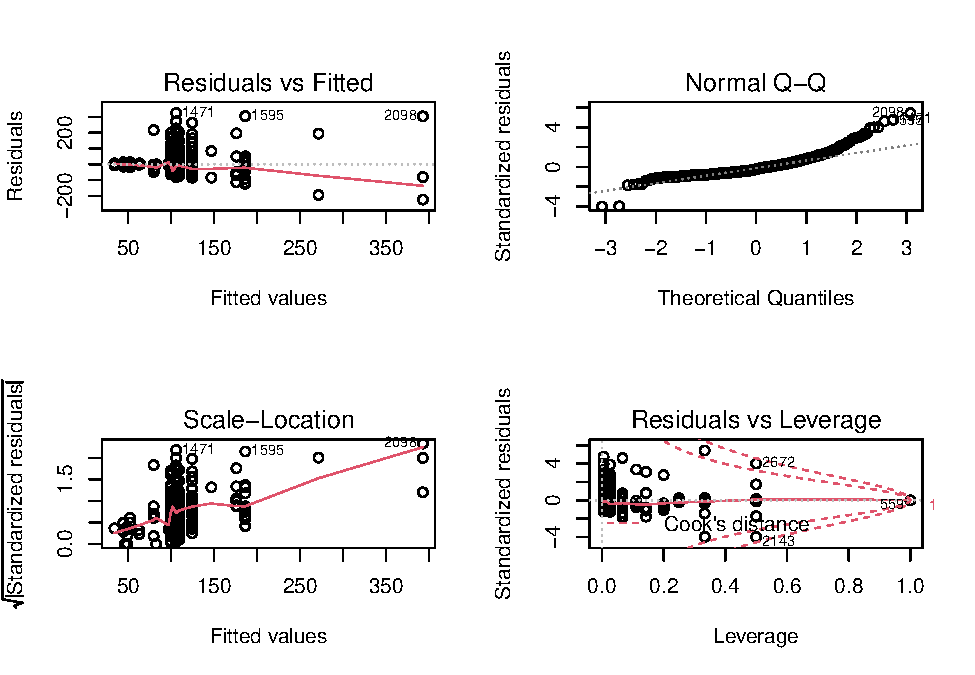
\includegraphics{Project_Code_files/figure-latex/q-2 residual-1.pdf}
\caption{Residual Plots for Question 2}
\end{figure}

\newpage

Below, average mail tail length by mating system and display system.

\begin{figure}
\centering
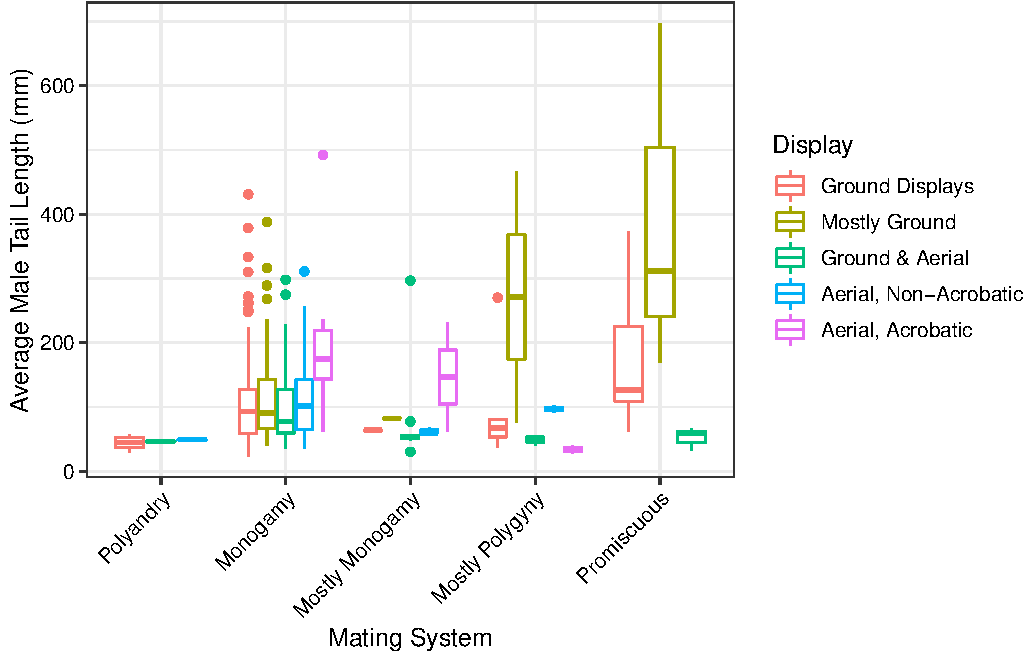
\includegraphics{Project_Code_files/figure-latex/q-2-plots-1.pdf}
\caption{Male Tail Length vs Mating Tactics}
\end{figure}

\newpage

Below, the same results as the previous page but with the mating system
and display system swapped.

\begin{figure}
\centering
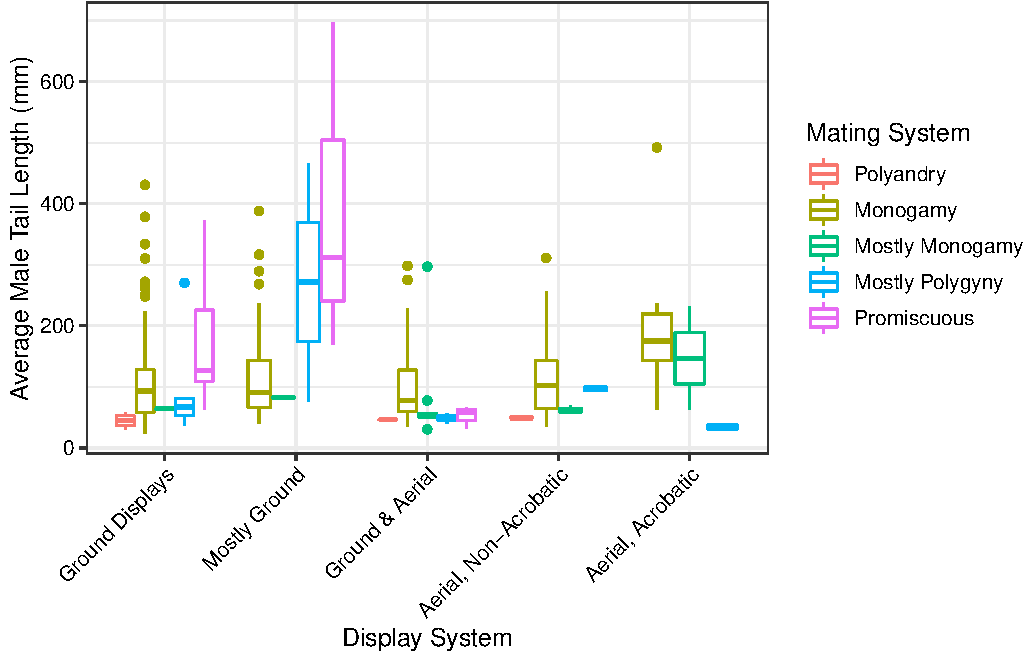
\includegraphics{Project_Code_files/figure-latex/q-2-plots2-1.pdf}
\caption{Male Tail Length vs Mating Tactics}
\end{figure}

\newpage

\hypertarget{summary-and-conclusions}{%
\section{Summary and Conclusions}\label{summary-and-conclusions}}

\emph{Summarize your major findings from your analyses in a few
paragraphs. What conclusions do you draw from your findings? Relate your
findings back to the original research questions and rationale.}

\hypertarget{part-1}{%
\subsection{Part 1}\label{part-1}}

The interaction between female mass and tail size predicts clutch size
(p \textless{} 0.001, n = 1642, R\textsuperscript{2} = 0.022). In
general, clutch size appears to decrease with increasing tail length,
but this effect is mediated by overall body size as expressed by mass.

Limitations (do we need to run more assumption tests for this one?) * R2
is low - model doesn't explain very much of the variance * residuals
plots - ?

This finding supports our hypothesis that birds with longer tails may
expend more resources collecting food because of their reduced agility
and therefore can raise smaller broods. More research is needed to
substantiate this hypothesis as well as to better understand how overall
body size mediates the effect.

\hypertarget{part-2}{%
\subsection{Part 2}\label{part-2}}

Mating system and display system together predict tail length (n = 476,
is the p-value just the interaction p-value for this one?)

Limitations, Part 2 * tail is not normally distributed (consider
transforming) * groups do not have equal variance (especially not
surprising with Mating System because the vast majority of the bird
species are Type 2 - Monogamous). * residual plots - ?

\newpage

\hypertarget{references}{%
\section{References}\label{references}}

Evans, M.R. 1999. The consequences of flight for the evolution of tail
ornaments in birds. In: Adams, N.J. \& Slotow, R.H. (eds) Proc. 22 Int.
Ornithol. Congr., Durban: 1823-1843. Johannesburg: BirdLife South
Africa.

Lislevand, T., Figuerola, J., and Székely, T. 2007. Avian body sizes in
relation to fecundity, mating system, display behavior, and resource
sharing. Ecology 88:1605.

\end{document}
